\documentclass{article}
\usepackage{graphicx}
\usepackage{epstopdf}
\usepackage{float}
\usepackage{amsmath}
\usepackage{multicol}
%\usepackage{enumerate}
\usepackage{graphicx}
\usepackage{color}
\usepackage[utf8]{inputenc} 
\usepackage[portuguese]{babel}
\usepackage[font=normalsize,format=plain,labelfont=bf,up,textfont=up,figurename=Figura,tablename=Tabela]{caption}
\usepackage{subcaption}
\usepackage[top=1in, bottom=1in, left=1.25in, right=1.25in]{geometry}
\usepackage{indentfirst}
\usepackage{fancyhdr}

% Font packages
\usepackage{amssymb}
\usepackage{amsfonts}
\usepackage{steinmetz}
% Nice extra font package, e.g. \mathds{1}
\usepackage{dsfont}


% Use multiple rows when writing tables
\usepackage{multirow}
\usepackage{booktabs}
\usepackage{bigstrut}
    \setlength\bigstrutjot{3pt}

% Uncomment next line to make footnots per page
\usepackage{perpage}

% Uncoment next group of lines to create the table of contents for the PDF
\usepackage{hyperref}
\definecolor{darkblue}{rgb}{0,0,0.5}
\hypersetup{
    pdftitle={Título},
    pdfauthor={Lucas Canto},
    bookmarksnumbered=true,     
    bookmarksopen=true,         
    bookmarksopenlevel=1,       
    colorlinks=true,
    linkcolor=darkblue,
    filecolor=darkblue,  
    urlcolor=darkblue,  
    citecolor=darkblue,              
    pdfstartview=Fit,           
    pdfpagemode=UseOutlines,    % this is the option you were lookin for
    pdfpagelayout=TwoPageRight
}

\renewcommand{\title}{House Prices - Machine Learning}
\newcommand{\subtitle}{Tópicos Especiais em Sistemas de Controle}
\pagestyle{fancy}
\fancyhead[L]{\title}
\fancyhead[R]{\subtitle}
\fancyhead[C]{\thepage}
\fancyfoot[C]{}

\allowdisplaybreaks

\renewcommand{\labelitemi}{\scalebox{0.8}[0.8]{$\bullet$}}
\newcommand{\tab}{\hspace{0.5cm}}

\definecolor{lightyellow}{rgb}{1,0.9568,0.8039}
\definecolor{mygreen}{rgb}{0, 0.35, 0}
\definecolor{myblue}{rgb}{0,0,1}

\begin{document}
\large
\begin{titlepage}
\begin{center}

% Upper part of the page. The '~' is needed because \\
% only works if a paragraph has started.
\rule{\linewidth}{0.5mm}\\[0.4cm]
{\huge Universidade Federal do Rio de Janeiro}
\rule{\linewidth}{0.5mm}\\[0.4cm]
\vspace{5mm}

\includegraphics[width=0.3\textwidth]{../img/minerva3}~\\[1cm]

% Title
{ \huge \bfseries \title \\[0.4cm] }

\textsc{\Large \subtitle}\\[2cm]

% Author and supervisor
\begin{minipage}{0.4\textwidth}
\begin{flushleft} \large
{Aluno:\\ Lucas Gama Canto \\ DRE: 113114241 \\Id do Kaggle: lucascanto}\\
%NOME DOS ALUNOS

\end{flushleft}
\end{minipage}
\begin{minipage}{0.4\textwidth}
\begin{flushright} \large
{Professor:\\ Heraldo Luís Silveira de Almeida, D.Sc.}\\
%Professor
\end{flushright}
\end{minipage}

\vfill

% Bottom of the page
{\large \today}

\end{center}
\end{titlepage}

\section{Introdução}
	\paragraph{}Este trabalho se baseia na implementação de uma estratégia de aprendizado de máquina com o intuito de gerar uma estimativa do preço das casas da cidade de Ames, Iowa nos Estados Unidos. O problema partiu de uma competição do \textit{Kaggle} denominada \textit{House Prices: Advanced Regression Techniques} e além da composição deste relatório, a estimativa alcançada no final foi enviada ao site para que esta pudesse ser avaliada e alocada no rank da competição.
	
	\paragraph{}Este relatório irá abranger desde o pré-processamento dos parâmetros de treino e teste disponíveis no \textit{Ames Housing dataset}, fornecido pelo próprio Kaggle, até a escolha do método de validação cruzada, técnica de minimização de erro, treino e predição da variável alvo, ou seja, os preços das casas de Ames.
	
	\paragraph{}O código foi desenvolvido em \textit{python} e executado no \textit{Spyder}, utilizando bibliotecas de computação científica, machine learning e manipulação de dados como \textit{numpy}, \textit{pandas} e \textit{scikit-learn}.

\section{Pré-processamento de Dados}
	\paragraph{}O pré-processamento dos dados de treino e teste se mostram como uma importante etapa da implementação do aprendizado. A ideia é de tratar ou transformar estes dados de forma que estes se tornem mais propensos a serem analisados como variáveis dependentes do objetivo.
	
	\paragraph{}Como já informado, a variável objetivo no problema é o preço das casas, denominado nos dados de treino como SalePrice. As variáveis dependentes se resumem em valores numéricos e categóricos que representam atributos físicos, espaciais e geográficos da casa, estas informações variam desde a área em metros quadrados do porão e do primeiro andar da casa até o número de piscinas e qualidade geral do imóvel. Informações mais detalhadas sobre estas variáveis dependentes podem ser encontradas no arquivo \textit{data\_description.txt} fornecido pelo Kaggle. No total existem 80 variáveis dependentes à disposição de processamento.
	
	\paragraph{}A etapa de pré-processamento se dividiu em 4 etapas:
	\begin{itemize}
		\item Verificação de variáveis com maior correlação ao preço
		\item Remoção de \textit{Outliers}
		\item Preenchimento ou exclusão de dados nulos
		\item Normalização de variáveis
	\end{itemize}
	
		\subsection{Matriz de Correlação}
		\paragraph{}De modo a limitar o espaço amostral e restringir algumas etapas do pré-processamento apenas à variáveis que possuam uma relação mais direta à variável objetivo, a matriz de correlação das variáveis dependentes em relação ao preço foi analisada.
		
		\begin{figure}[h]
			\centering
			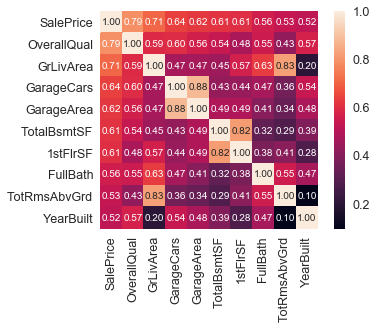
\includegraphics[scale=0.9]{../img/correlation}
			\caption{Matriz de correlação das 10 variáveis mais correlatas a SalePrice}
		\end{figure}
		
		\paragraph{}É possível verificar que quase todas as variáveis verificadas como as mais correlatas se apresentam como numéricas, com a exceção de \textit{OverallQual} que coincidentemente também se apresentou como a variável mais correlata.
		
		\paragraph{}Como \textit{OverallQual} se trata de uma variável categórica, esta variável não irá ser modificada nas etapas de relação de outliers e normalização, visto que isto poderia acarretar na perda de possíveis dados importantes para o treino da estratégia.
		
		\paragraph{}Outro fator a ser analisado é a semelhança de valores de correlação entre variáveis dependentes, isto indica que não há necessidade de utilizar duas variáveis com o mesmo grau de correlação pois elas possivelmente tem um comportamento semelhante perante a variável objetivo. Pares de variáveis como \textit{GarageCars} e \textit{GarageArea}, \textit{TotalBsmtSF} e \textit{1stFloor}, \textit{TotRmsAbvGrd} e \textit{GrLivArea} se encaixam nessa característica.
		
\section{Treinamento e Previsão}
	\paragraph{}Teste.
	
\section{Conclusão}

	\paragraph{}Teste.

\end{document}